\clearpage
\subsection{Система с переменной структурой  со скользящим режимом движения} \label{title:VSS_SDM}
Наиболее рациональной считается идея синтеза систем с переменной структурой с искусственным вырожденным движением. Сущность этого подхода заключается в следующем. Как и прежде считается, что имеется несколько линейных структур, не обязательно  устойчивых, из которых синтезируется система с переменной структурой. В фазовом пространстве искусственно задается  некоторая  гиперплоскость S, движение в которой обладает желаемыми свойствами, причем траектории, лежащие  в этой плоскости, не принадлежат ни одной из линейных структур. Последовательность изменения структур должна быть выбираема такой, чтобы изображающая  точка при любых начальных условиях всегда попадала на эту плоскость, а затем двигалась (скользила) по ней. Тогда с момента попадания  на эту гиперплоскость в системе будет существовать искусственное вырожденное движение, которое можно наделить рядом полезных свойств, не принадлежащих ни одной из фиксированных структур. 

Для рассмотренной ранее СПС с устойчивым вырожденным движением, которое определяется уравнением  \eqref{eq:straight_S1} введем на фазовой плоскости линию скольжения  \eqref{eq:straight_sliding}. Все остальные параметры управляющего устройства  оставим без изменений.
 Угол наклона у линии скольжения меньше угла наклона сепаратрисы седловой траектории с отрицательным наклоном в 2 раз. Если сделать угол наклона больше, то скольжения наблюдаться не будет.
\begin{equation}
    \begin{aligned} \label{eq:straight_sliding}
       S&=x_2-\tau\,x_1=0\\
       S&=x_2+0.5\,x_1=0\\
    \end{aligned}
\end{equation}

Структурная схема системы с переменной структурой со скользящим режимом движения имеет тот же вид, что и на рис.\ref{fig:sim_VSS_steady_degenerate_motion}, только в переменную p блока Gain вставляем значение угла наклона у линии скольжения.

Исследуем движение фазовых координат во времени посредством моделирования процессов в системе при отклонении системы от состояния равновесия. Фазовые траектории в системе на рис.\ref{fig:VSS_steady_degenerate_motion_ft_SLM}. 
В дополнение на рис.\ref{fig:VSS_steady_degenerate_motion_sv_SLM} указано изменение выходной переменной и её производной. 
\begin{figure}[!h]\centering
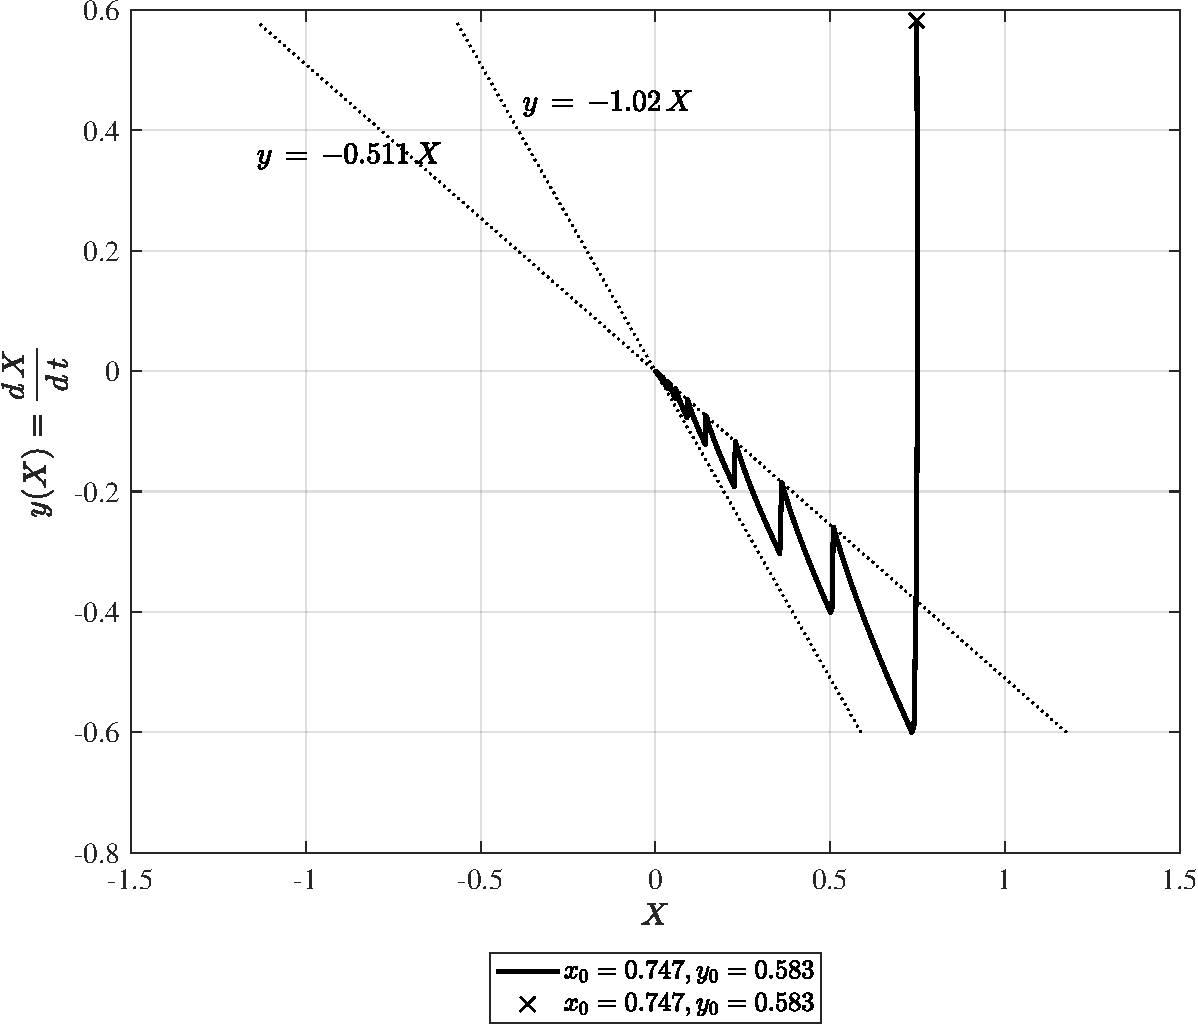
\includegraphics[width=1.0\linewidth]{images/VSS_steady_degenerate_motion_ft_SLM}
\caption{ Фазовые траектории для системы с переменной структурой с разными начальными условиями.}\label{fig:VSS_steady_degenerate_motion_ft_SLM}
\end{figure}
\begin{figure}[!h]\centering
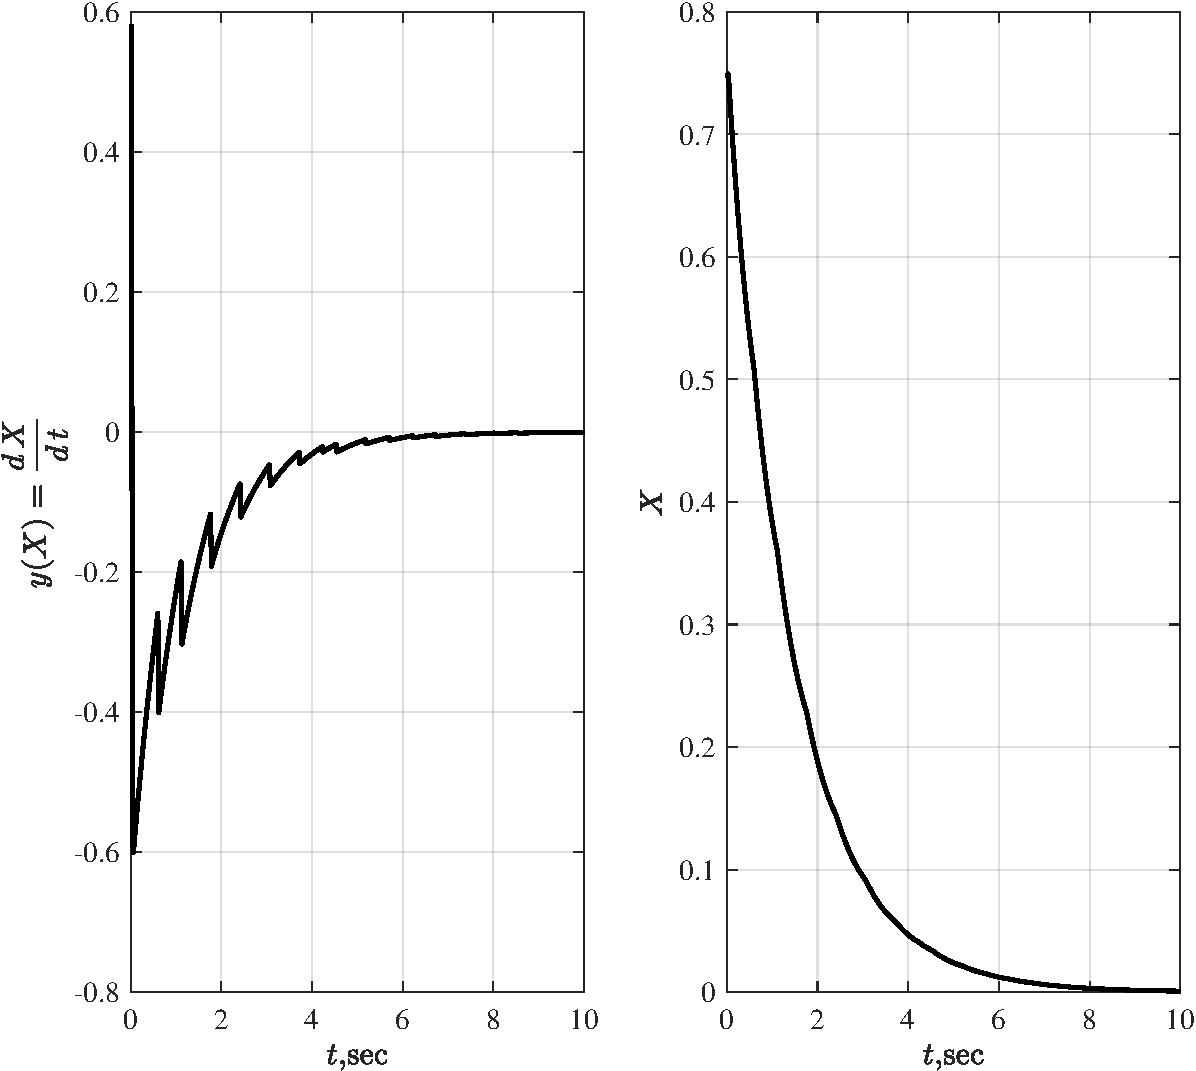
\includegraphics[width=1.0\linewidth]{images/VSS_steady_degenerate_motion_sv_SLM}
\caption{ Графики изменения выходной переменной и её производной.}\label{fig:VSS_steady_degenerate_motion_sv_SLM}
\end{figure}

Видно, что СПС дают существенно лучшие показатели по сравнению с линейными системами регулирования. Как видно из полученных графиков в СПС без вырожденного устойчивого движения и в СПС с вырожденным устойчивым движением существуют колебания, а в СПС со скользящим режимом колебания отсутствуют. Изменяя целенаправленно параметры СПС, можно влиять на качественные показатели системы. 

Таким образом, подводя итоги, можем отметить, что СПС может быть построена по одному из трех рассмотренных выше принципов. В большинстве случаев предпочтение отдается системам со скользящим режимом в силу их специфических свойств.
